%\documentclass[tikz,convert={outfile=\s1.svg}]{standalone}
\documentclass[tikz]{standalone}
\usepackage{amsthm}
\usepackage[landscape]{geometry}
\usepackage{multicol}
\usepackage{tikz}
\usepackage{pgfplots}
\usepackage{xcolor}
\usepackage{amsmath}
\usepackage[T1]{fontenc}
\usepackage{utopia}
\usepackage{changepage}
\usepackage{amssymb}
\usepackage{fancyhdr}
\usepackage[many]{tcolorbox}
\usepackage{moresize}
\usepackage{fullpage}
\usepackage{mathpazo}
\usepackage{tikz-3dplot}
\usepackage{cancel}
\tdplotsetmaincoords{70}{165}
\pgfplotsset{compat=1.18}
\usepackage{enumitem}
\usepackage{tabularray}
\usepackage{mathtools}

\UseTblrLibrary{diagbox}

\usetikzlibrary{
    shadings, calc, patterns, angles, quotes, arrows.meta, 
    decorations.pathmorphing, decorations.pathreplacing, 
    fadings, 3d, perspective, backgrounds, intersections, 
    decorations.markings, bending, positioning, 							spy,shapes.geometric,shadows,shapes.symbols, fadings, matrix, fit
}

\usepgfplotslibrary{
    groupplots, external, colormaps, patchplots, fillbetween
}


% Reds (r)
\definecolor{r1}{RGB}{255, 191, 191}    % Light coral
\definecolor{r2}{RGB}{255, 191, 223}    % Light pink
\definecolor{r3}{RGB}{255, 207, 207}    % Light rose

% Blues (b)
\definecolor{b1}{RGB}{191, 223, 255}    % Light blue
\definecolor{b2}{RGB}{191, 239, 255}    % Light sky
\definecolor{b3}{RGB}{191, 255, 255}    % Light cyan

% Greens (g)
\definecolor{g1}{RGB}{191, 255, 191}    % Light green
\definecolor{g2}{RGB}{191, 255, 223}    % Light mint
\definecolor{g3}{RGB}{207, 255, 207}    % Light sage

% Oranges (o)
\definecolor{o1}{RGB}{255, 223, 191}    % Light peach
\definecolor{o2}{RGB}{255, 239, 191}    % Light cream
\definecolor{o3}{RGB}{255, 231, 191}    % Light buff

% Violets (v)
\definecolor{v1}{RGB}{223, 191, 255}    % Light purple
\definecolor{v2}{RGB}{239, 191, 255}    % Light lilac
\definecolor{v3}{RGB}{231, 191, 255}    % Light lavender

% Yellows (y)
\definecolor{y1}{RGB}{255, 255, 191}    % Light yellow
\definecolor{y2}{RGB}{255, 247, 191}    % Light cream yellow
\definecolor{y3}{RGB}{255, 239, 191}    % Light warm cream

\definecolor{w}{HTML}{eeeeee}
\definecolor{g}{HTML}{444444}
\definecolor{b}{HTML}{222222}
\definecolor{lightgrey}{HTML}{cccccc}
\definecolor{firebrick}{RGB}{178, 34, 34}
\definecolor{myg}{RGB}{3, 252, 177}


\color{w}
\begin{document}
\ssmall
%\pagecolor{b}
\nopagecolor
\fontfamily{put}

		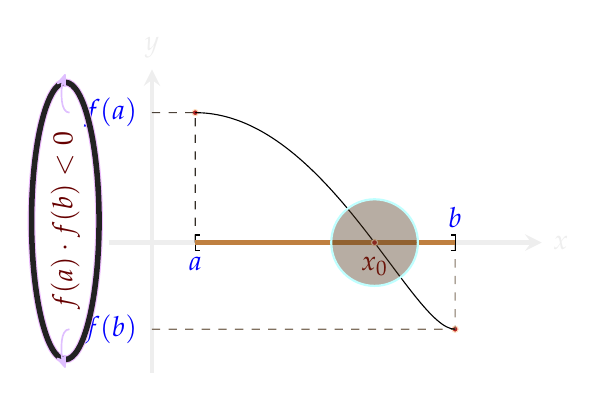
\begin{tikzpicture}[scale =0.55]
				\coordinate (A) at (-1, 3);
				\coordinate (B) at (5, -2);
				\coordinate (O) at (-2, 0);
				
				\draw[draw=w, ultra thick, -stealth] (-3, 0) -- (7, 0) node[text=w, right] {$x$};
				\draw[draw=w, ultra thick, -stealth] (-2, -3) -- (-2, 4) node[text=w, above] {$y$};		
			
				\filldraw[draw=o1, fill=firebrick] (A) circle (2pt);
				\filldraw[draw=o1, fill=firebrick] (B) circle (2pt);	
			
				\coordinate (Ax) at (A |- O);
				\coordinate (Ay) at (A -| O);
				
				\coordinate (Bx) at (B |- O);
				\coordinate (By) at (B -| O);
				
				\draw[dashed, draw=o1!20!black] (Ax) -- (A);
				\draw[dashed, draw=o1!30!black] (Ay) -- (A);
				\node[left, outer sep=2pt, text=blue] (ay) at (Ay) {$f(a)$};
				\node[below, outer sep=2pt, text=blue] at (Ax) {$a$};
				
				\draw[dashed, draw=o1!50!black] (Bx) -- (B);
				\draw[dashed, draw=o1!50!black] (By) -- (B);
				\node[left, outer sep=2pt, text=blue] (by) at (By) {$f(b)$};
				\node[above, outer sep=2pt, text=blue] at (Bx) {$b$};
				
				\draw[thin, draw=black] ($(Ax) + (3pt, -5pt)$) -- ++(180:3pt) -- ++(90:10pt) -- ++ (0:3pt);
				\draw[thin, draw=black] ($(Bx) + (-3pt, -5pt)$) -- ++(0:3pt) -- ++(90:10pt) -- ++ (180:3pt);				
				\draw[ultra thick, draw=brown] (Ax) -- (Bx);
				
				\draw[] (A) .. controls +(0:3cm) and +(left:1cm) .. (B); 
				\coordinate (X) at ($(Ax)!.69!(Bx)$);
				\filldraw[draw=o1, fill=firebrick] (X) circle (2pt);
				\node[below, outer sep=2pt, text=red!50!black] at (X) {$x_0$};
						
				\coordinate (F) at ($(Ay)!0.5!(By) + (-2, 0)$);
				\node[shape=ellipse, double=b, double distance=2pt, draw=v2, rotate=90, text=red!40!black, outer sep=3pt] (ff) at (F) {$f(a)\cdot f(b) < 0$};				
				\draw[->, draw=v1, >={Stealth[round]},semithick] (ay) to[out=180, in=90] (ff.east);
				\draw[->, draw=v1, >={Stealth[round]},semithick] (by) to[out=180, in=270] (ff.west);	
				
				\filldraw[draw=b3, thick, fill=brown!40!black, fill opacity=0.4] (X) circle (1cm);
			\end{tikzpicture}

\end{document}